%*****************************************
\chapter{Word Embeddings for Misinformation Detection}\label{ch:word-embeddings}
%*****************************************

\section{Background}
\label{sec:3-background}

One of the prevailing approaches to solving tasks in \ac{NLP} is based on the hypothesis that words which appear in close proximity tend to have a similar meaning.\sidecite{Levy:2014} This is known as the \emph{distributional hypothesis} and was originally posited in 1954.\sidecite{Harris:1954} The distributional hypothesis has since led to the development of various methods to encode text in numeric form. Building on it, distributed representations for computing elements were introduced by \citeauthoryear{Hinton:1986} about three decades later. They were among the first to create numerical representations of words.

More recent approaches in \ac{NLP} problem-solving are based on neural network word embedding.\sidenote{\citeauthoryear{Collobert:2008}, \citeauthoryear{Mikolov:2013}} These models are constructed using neural nets that represent the similarity between words using dense continuous, real vectors of numbers. Today, the representations of words as vectors are generally referred to as \emph{word embeddings}.\sidecite{Levy:2014} Semantically similar words will have numerically similar vectors—known as learned distributed feature vectors—which ideally have a much smaller dimension than the vocabulary. Embeddings can also be generated for whole sentences by aggregating word embeddings or using neural nets trained specifically for this task. When the dimensions of the learned vectors of words are reduced to two or three and visualised on a Cartesian plane, relationships between them become apparent. In this chapter, experiments were set up using word and sentence embeddings to find semantic differences between reactions to rumours and non-rumours. The experimental procedure, results, and conclusions are explained in the following subsections.

\section{Related work}
\label{sec:3-related-work}

Word embedding models have shown a better performance than classical methods, such as \ac{BoW}, Term Frequency-Inverse Document Frequency and Distributional Embeddings.\sidenote{\citeauthoryear{Mikolov:2011}, \citeauthoryear{Mikolov:2013}} However, according to \citeauthoryear{Goldberg:2014}, it remains unknown exactly why some models produce good word representations. Word embeddings have been used effectively for fake news detection, as demonstrated by \citeauthoryear{Bhattacharjee:2018}, \citeauthoryear{Shang:2018} and \citeauthoryear{Shu:2019}. They have also been used for automated fact-checking.\sidecite{Konstantinovskiy:2018}

\citeauthoryear{Mikolov:2013} observed that a limitation of word representations is their inability to capture idioms. For example, the phrase `Washington Post' refers to a newspaper, and its meaning is not directly deducible by simply combining the individual meanings of the words `Washington' and `Post'. They, therefore, suggest using a Skip-gram model\sidecite{Mikolov:2013b} to learn vector representations, as such a model is capable of representing phrases as vectors and is highly efficient, in terms of training time and accuracy. Nonetheless, word embeddings are now established and have been successfully applied to improve performance in various \ac{NLP} tasks.\sidecite{Collobert:2011} Examples of open-sourced word embedding tools include \texttt{word2vec} by \citeauthoryear{Mikolov:2013}, Global Vectors for Word Representation (or \texttt{GloVe}) by \citeauthoryear{Pennington:2014}, and \texttt{FastText} by \citeauthoryear{Bojanowski:2016}. Word embeddings have effectively been used for fake news detection. Some papers which used these latent text features are listed in \autoref{tab:mlformisinfo}, in \sectionref{sec:2-text}.

\newthought{False news and} rumour content tend to be semantically distinct from authentic or non-rumour content.\sidenote{\citeauthoryear{Parikh:2018}, \citeauthoryear{Potthast:2018}} The observation that the semantics of the two tend to differ partly motivates this investigation. Additionally, \citeauthoryear{Choi:2020} found that echo chambers tend to increase virality and accelerate the spread of rumours. They define an echo chamber as a collection of users that have shared at least two rumours in common. They analysed more than one hundred rumours from six fact-checking platforms. These rumours were the subject of nearly 300,000 tweets made by over 170,000 users. Therefore, it can be argued that those who retweet rumours are likely to be more driven to amplify a common message, than those who retweet non-rumour tweets. This amplification may also be in the form of replies that express agreement and may, therefore, be semantically similar.

The experiment presented in this chapter differs from some previous studies\sidenote{\citeauthoryear{Wu:2015}, \citeauthoryear{Zhang:2016}, \citeauthoryear{Zhang:2017}}—it focuses not on the rumours or non-rumours posted, but on the reactions which they attract. The goal here is to find out whether there is a difference in dispersion between people’s reactions to rumours and non-rumour in tweets. Note that in this section, `reactions' and `comments' refer to the replies received by tweets.

\section{Problem definition}
\label{sec:3-problem}

In this experiment, the aim is to determine whether or not there is any evidence to differentiate between rumours and non-rumours tweets, based on the reactions they receive. Latent text representations are used as the discriminant between the two groups. This study is carried out using statistical hypothesis testing. The hypotheses can be stated as follows:

\begin{hyp}
  [Null] \label{hyp:a}\textit{the semantic similarities between rumour and non-rumour tweet reactions are equal.}
\end{hyp}
\begin{hyp}
  [Alternative] \label{hyp:b}\textit{the semantic similarities of rumour tweet reactions are greater than those of non-rumour tweet reactions.}
\end{hyp}

For both \Cref{hyp:a,hyp:b}, the semantic similarities are measured using \texttt{InferSent}\sidecite{Conneau:2017} sentence embeddings. It is expected that there will be a greater similarity amongst rumour tweet reactions, compared with non-rumours ones. This is in line with the aforementioned observations. The method through which \Cref{hyp:b} will be tested against \Cref{hyp:a} is explained in the next section.

\section{Methodology and materials}
\label{sec:3-methodology}

\subsection{Experimental procedure}
\label{ssec:3-experimental-procedure}

Let $P_{ALL} \in \left\{ P^R, P^F \right\}$ represent a dataset containing all $M$ rumour $N$ and non-rumour (factual) posts, $P^R = \left\{ p_1^R, \ldots, p_M^R \right\}$ and $P^F = \left\{ p_1^F, \ldots, p_N^F \right\}$, respectively. Each rumour post $p_i^R$ has received comments $c_i^R = \left[c_{i,1}^R, c_{i,2}^R , \ldots, c_{i,m_i}^R \right]$, where $m_i$ is the total number of comments that follow, and $i = \{1 \ldots M\}$. Likewise, each factual tweet $p_i^F$ has received $c_i^F = \left[c_{i,1}^F, c_{i,2}^F, \ldots, c_{i,n_i}^F \right]$ comments (a total of $n_i$), with $i = \{1 \ldots N\}$. Therefore, $C^R = \bigcup\limits_{i=1}^M c_i^R$ and $C^F = \bigcup\limits_{i=1}^N c_i^F$ are all the reactions to rumours and non-rumours, respectively. Algorithm \autoref{3-infersent} summarises the computations for this experiment.

Before the experiment, the data was cleaned as follows: (i.) all datasets were cleaned to remove usernames and hashtags; (ii.) comments less than three words long were removed.\sidenote{This helps to make the word embedding more accurate. A post may have only a single comment, but all comments must be more than three words long, or else that post is excluded.} Next, a	pre-trained \texttt{InferSent} word embedding model was used to generate 4096-length vectors for each rumour and non-rumour reaction. This gives us matrices for rumour and non-rumour embeddings, $E^R = (e_{i,j}) \in \mathbb{R}^{M \times 4096}$ and $E^F = (e_{i,j}) \in \mathbb{R}^{N \times 4096}$, respectively.

\newthought{The average pairwise} cosine similarities, $cs_{avg}$, between the embeddings for rumour and non-rumour reactions are separately calculated. Self-comparisons between items (having a similarity of $1$) are excluded. Therefore, an $l \times 4096$ matrix of embeddings is inputted and the output is a $l$-length vector in return,\sidenote{The row-wise mean is calculated first in Line 6 of Algorithm \autoref{3-infersent} to compare each comment with every other comment except itself.} after finding the mean. In this vector, each item is the mean of cosine distances between the embedding of a comment and all other comments.

Lastly, the average of each vector is calculated, as $A^R$ and $A^F$, and the difference between the two is found as $\Delta A = A^R - A^F$. The higher $\Delta A$ is, the more similar rumours are as compared with non-rumours, and vice versa.

\begin{algorithm}
\caption{Comparison of rumour and non-rumour comments using \texttt{InferSent} embeddings}\label{3-infersent}
\begin{algorithmic}[1]
\Require Comments $C^R$ and $C^F$
\Ensure $\Delta A$
\item[]
\Function{InferSentEmbed}{$text$}
  \State\Return \texttt{InferSent} embedding vector for $text$, $\mathbf{e}$ \Comment{$|\mathbf{e}| = 4096$}
\EndFunction
\Function{PairwiseCosSim}{$\bm{X} = (e_{i,j}) \in \mathbb{R}^{l \times 4096}$}
  \State Pairwise cosine similarity matrix for $\bm{X}$ is $\bm{S} = (a_{i,j}) \in \mathbb{R}^{l \times l}$
  \State\Return $mean(S)$ \Comment{do row-wise mean first}
\EndFunction
\ForAll {$c_i \in C^F$}
  \State $\bm{E_i^F}$ = \Call{InferSentEmbed}{$c_i$}
\EndFor
\ForAll {$c_i \in C^R$}
  \State $\bm{E_i^R}$ = \Call{InferSentEmbed}{$c_i$}
\EndFor
\State $E^F = \left\{ E_1^F, \ldots, E_M^F \right\} = (e_{i,j}) \in \mathbb{R}^{M \times 4096}$
\State $E^R = \left\{ E_1^R, \ldots, E_N^R \right\} = (e_{i,j}) \in \mathbb{R}^{N \times 4096}$

\State $\bm{A^F}$ = \Call{PairwiseCosSim}{$E^F$}
\State $\bm{A^R}$ = \Call{PairwiseCosSim}{$E^R$}

\State $\Delta A = A^R - A^F$
\State\Return $\Delta A$
\end{algorithmic}
\end{algorithm}

\texttt{InferSent} is trained on natural inference data and it generates semantic representations for sentences in English.\sidecite{Conneau:2017} Embeddings of phrases and sentences are typically obtained by averaging their constituting word embedding vectors. However, \texttt{InferSent} is advantageous because it takes the order of words into account to produce embeddings for whole sentences, as it is built on a \ac{RNN}.\sidenote{\citeauthoryear{Conneau:2017}, \citeauthoryear{Konstantinovskiy:2018}}

\subsection{Datasets}
\label{ssec:3-datasets}

The PHEME dataset created by \citeauthoryear{Zubiaga:2016b} was used to evaluate \Cref{hyp:a,hyp:b}. It contains nearly 6,000 tweets concerning five fatal incidents that occurred in North America and Europe between 2014 and 2015. A breakdown of this dataset is shown in \autoref{tab:3-pheme}.

\begin{table}[h]
\addlinespace
    \begin{tabularx}{\textwidth}{>{\raggedright}p{2.5cm}llll}
      \toprule
        \tableheadline{Event} &
        \tableheadline{Rumours} &
        \tableheadline{\shortstack[l]{Non- \smallskip\\ Rumours}} &
        \tableheadline{\shortstack[l]{Rumour \smallskip\\ Comments}} &
        \tableheadline{\shortstack[l]{Non-rumour \smallskip\\ Comments}} \\
      \midrule
        Charlie Hebdo Shooting (Jan. 2015) & 458 (22\%) & 1620 (78\%) & 422 (22.0\%) & 1493 (88\%) \\
        Ferguson Unrest (Aug. 2014) & 284 (24.8\%) & 231 (75.2\%) & 257 (25.8\%) & 740 (74.2\%) \\
        Germanwings Crash (Mar. 2015) & 238 (50.7\%) & 231 (49.3\%) & 160 (49.0\%) & 166 (51.0\%) \\
        Ottawa Shooting (Oct. 2014) & 470 (52.8\%) & 420 (47.2\%) & 426 (54.2\%) & 360 (45.8\%) \\
        Sydney Siege (Dec. 2014) & 522 (42.8\%) & 699 (57.2\%) & 486 (42.6\%) & 656 (57.4\%) \\
        \bottomrule
    \end{tabularx}
\caption{Breakdown of PHEME dataset}
\label{tab:3-pheme}
\end{table}

\subsection{Results and discussion}
\label{ssec:3-results}

The tendency for rumour and non-rumour content to differ semantically was introduced in \sectionref{sec:3-related-work}. This experiment hypothesises that rumour reactions will generally be similar to each other—rather than to non-rumour reactions—and vice versa. Similarity, here, is evaluated by computing and comparing the sentence embeddings of the two groups of tweets. It is expected, therefore, that the mean of the pairwise distances between rumours will generally be greater than that between non-rumour comments.

To verify this scientifically, a statistical test was carried out on the experimental results. The differences in the similarities of rumour and non-rumour reactions were evaluated using the Wilcoxon–Mann–Whitney test, at 5\% significance level. This test was chosen because the resulting data, for all datasets, did not pass the test for normality, and therefore, could not be assumed to be normally distributed. A Shapiro-Wilk test showed that the distribution of rumour and non-rumour similarity values departed significantly from a normal distribution (R — rumour, NR — non-rumour):
\begin{itemize}
  \item Charlie Hebdo: R ($W = 0.971, p < 0.01$), NR ($W = 0.915, p < 0.01$)
  \item Ferguson: R ($W = 0.890, p < 0.01$), NR ($W = 0.915, p < 0.01$)
  \item Germanwings: R ($W = 0.929, p < 0.01$), NR ($W = 0.970, p < 0.01$)
  \item Ottawa: R ($W = 0.914, p < 0.01$), NR ($W = 0.901, p < 0.01$)
  \item Sydney: R ($W = 0.918, p < 0.01$), NR ($W = 0.883, p < 0.01$)
\end{itemize}

Therefore, the differences between the median similarities, rather than the mean, were conclusively analysed, by applying the Wilcoxon–Mann–Whitney test.

\autoref{tab:3-results} summarises the results of this experiment, while detailed plots are presented in \autoref{fig:3-exp-1.2}. Recall from Algorithm \autoref{3-infersent}, that $A^R$ and $A^F$ are the mean similarities between rumour and non-rumour (factual) tweet reactions, respectively. $Med^R$ and $Med^F$ ($\Delta Med = Med^R - Med^F$) are the median similarities between rumours and non-rumours, respectively.

\begin{table}[h]
\addlinespace
    \begin{tabularx}{\textwidth}{Xllllllll} \toprule
        \tableheadline{Event} & \tableheadline{$A^R$} & \tableheadline{$A^F$} & \tableheadline{$\Delta A$} &  \tableheadline{$Med^R$} & \tableheadline{$Med^F$} & \tableheadline{$\Delta Med$} & \tableheadline{$p\textrm{-}value$} \\ \midrule
        Charlie Hebdo & 0.603 & 0.599 & 0.004 & 0.603 & 0.608 & -0.005 & 0.487 \\

        Ferguson & 0.632 & 0.617 & 0.015 & 0.629 & 0.618 & 0.012 & $\textrm{1.686} \times \textrm{10}^\textrm{-4}$ \\

        German- wings & 0.603 & 0.593 & 0.001 & 0.608 & 0.599 & 0.009 & 0.114 \\

        Ottawa & 0.615 & 0.613 & 0.002 & 0.614 & 0.604 & 0.009 & 0.136 \\

        Sydney & 0.606 & 0.614 & -0.008 & 0.607 & 0.616 & -0.009 & 0.998 \\

        \bottomrule
    \end{tabularx}
\caption{Summary of experimental and statistical results for comparisons between sentence embeddings.}
\label{tab:3-results}
\end{table}

\begin{figure}[h]
  \myfloatalign
  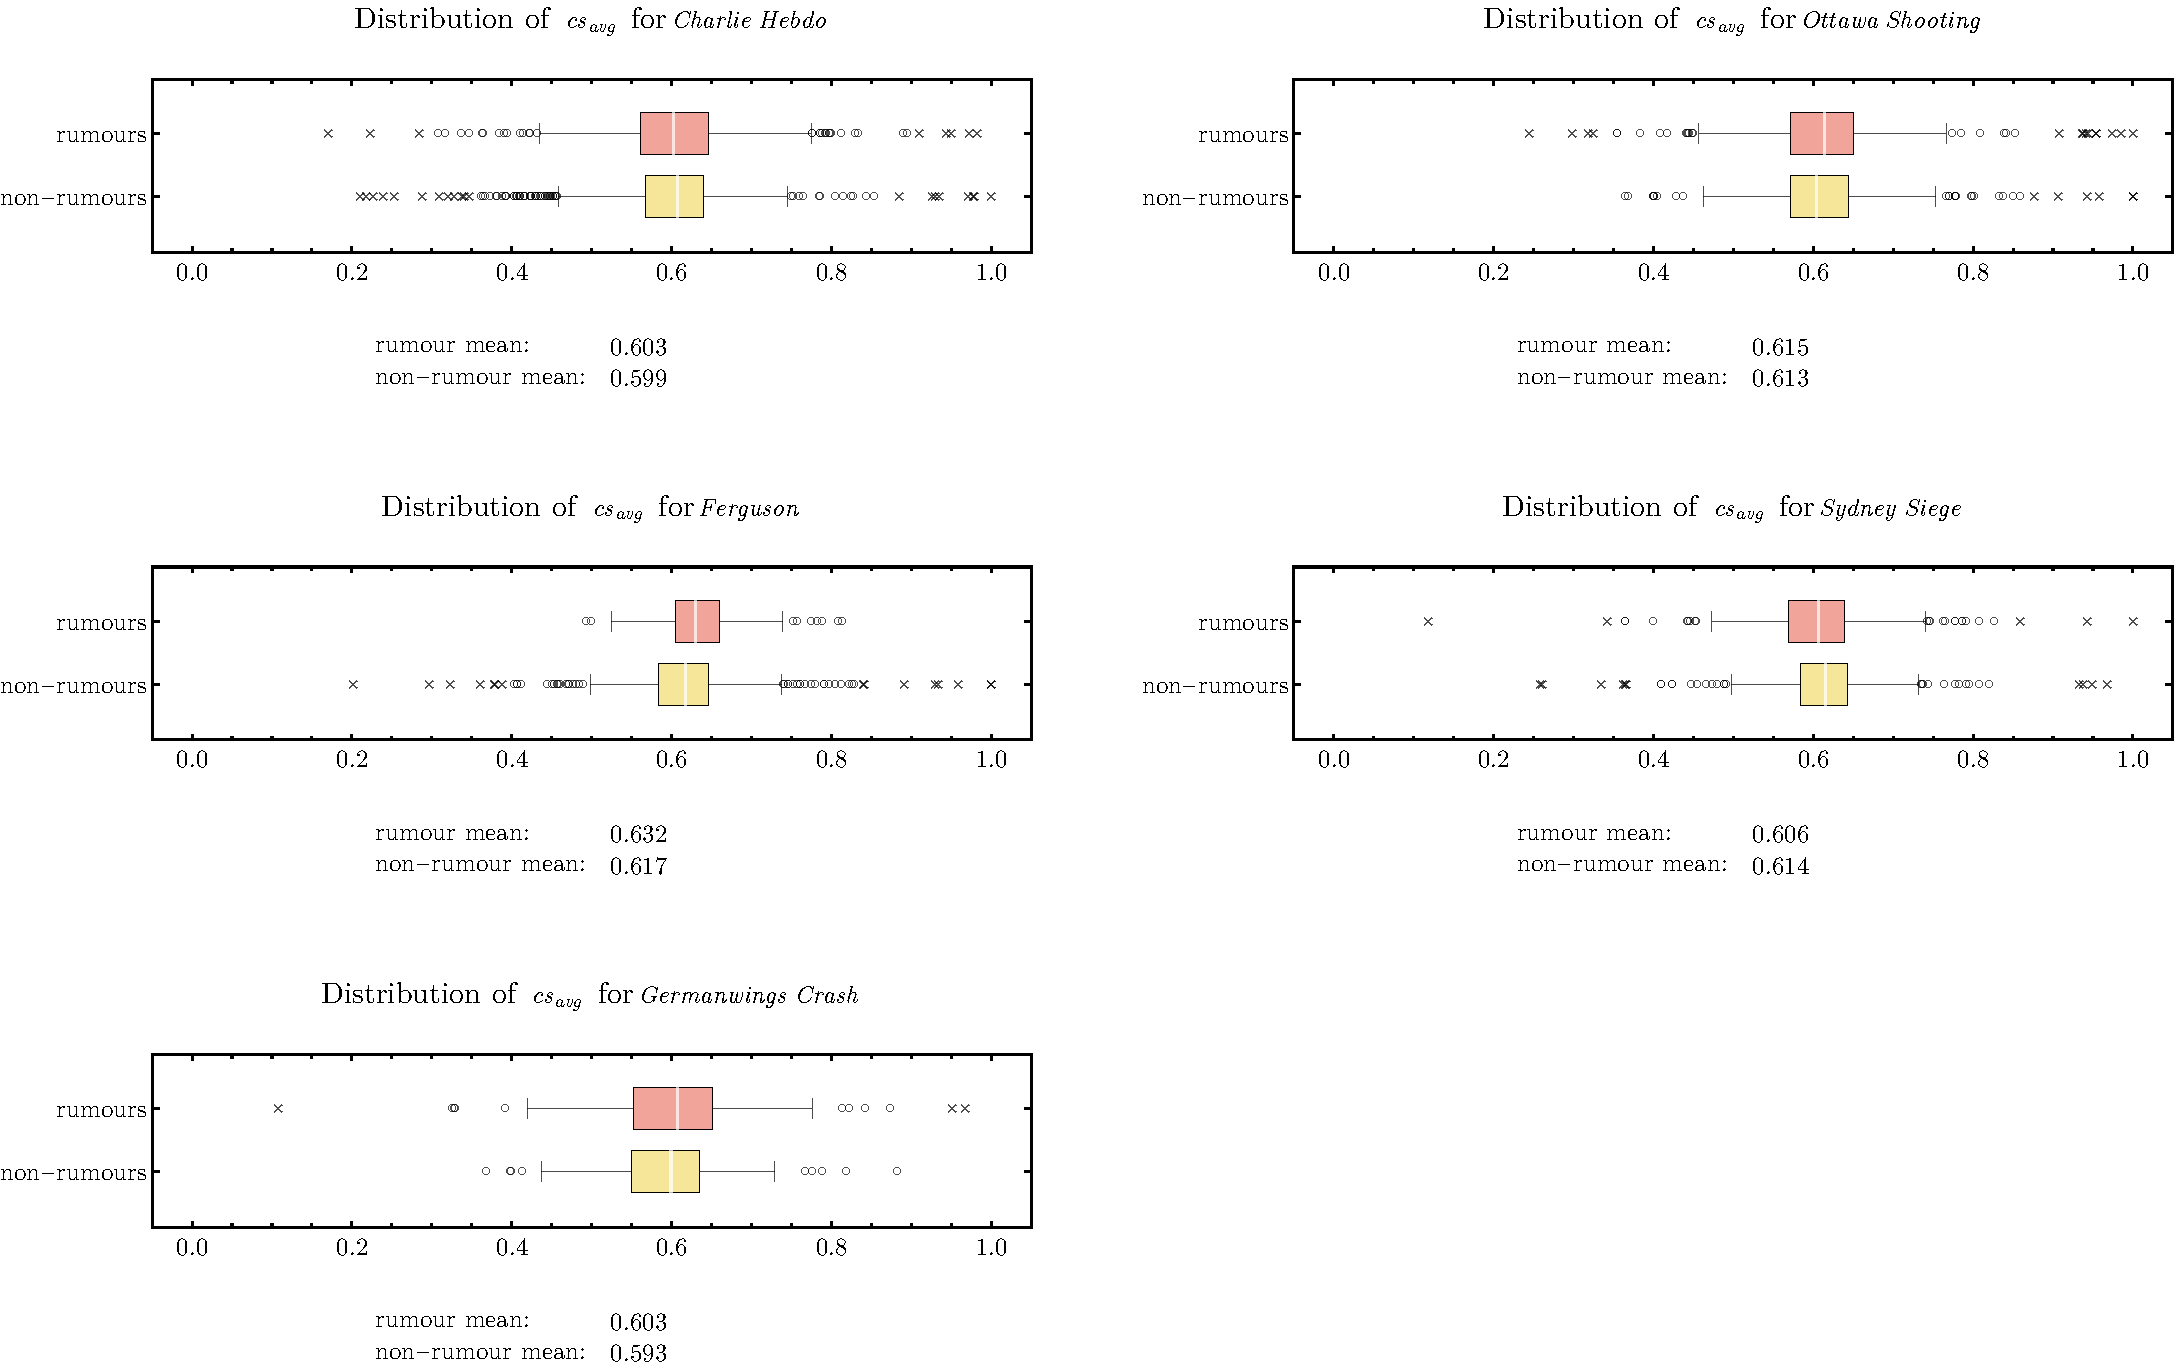
\includegraphics[width={\textwidth + \marginparsep + \marginparwidth}]{gfx/Experiment_1_2}
  % \begin{varwidth}{\textwidth + \marginparsep + \marginparwidth}
  \caption{Box plots of distributions of $cs_{avg}$ for rumour and non-rumour reactions.}
  % \end{varwidth}
  \label{fig:3-exp-1.2}
\end{figure}

The results show that there are no significant, consistent differences between rumours and factual comments when comparing the two using sentence embeddings. Most values of $\Delta A$ are positive as expected, except for the Sydney Siege dataset. The $\Delta Med$ values are also positive, except for the Charlie Hebdo and Sydney Siege datasets. The two measures may suggest that the rumour reactions are generally semantically more similar to each other than non-rumours, but $\Delta A$ and $\Delta Med$ indicate that such a conclusion cannot be made. Except for the Ferguson dataset, the null hypothesis (\Cref{hyp:a})—that the average semantic similarities between rumour and non-rumour tweet reactions are equal—is not rejected at the 5\% level, based on the Wilcoxon–Mann–Whitney test. Therefore, in summary, the \Cref{hyp:a} tested in this experiment is not rejected.

There are some possible factors which may have affected the outcome of this experiment. First, sentence embeddings work better with well-written sentences. However, short texts of just 140 characters—not necessarily forming complete sentences—were used here. Second, the datasets used are concerned with separate events in different countries, which may have been discussed in different ways. For example, the Charlie Hebdo event occurred in France, and some of the tweets in that dataset are in French. Similarly, the Germanwings Crash data contains some tweets in German. However, an \texttt{InferSent} model for English texts was used to get the sentence embeddings, as most of the tweets are in English. Lastly, the small size of the dataset, coupled with the imbalance of the number of examples in each class, possibly influenced the outcome of this experiment.

\newthought{Further experiments were} conducted with minor changes made to the methodology. In one of the follow-up studies, the aim was to determine whether rumour posts are more similar to the comments they attract, compared with non-rumours. In other words, the goal is to compare the semantic differences between rumours and their reactions, and non-rumours and their comments. The following steps were carried out, for each event:

\begin{itemize}
  \item Embed each post (rumour or non-rumour) into a 300-length vector.
  \item Embed its corresponding comments also into 300-length vectors.
  \item Find the averages of pairwise cosine similarities and Euclidean distances between each post and its set of comments. Here, $cs_{avg}$ represents the similarity between a post and the comments it attracted.
\end{itemize}

The results of this experiment (see \autoref{fig:3-exp-1.3}, \autoref{fig:3-exp-1.3e} and \autoref{tab:3-exp-1.3}) also did not yield conclusive results. They show that for some events, the rumour posts are more similar to their comments, while the opposite is the case for others. Even when the embeddings of the comments are averaged before being compared with the embeddings of their original post, significant differences were not found between rumour and non-rumour tweets.

\begin{figure}[h]
  \myfloatalign
  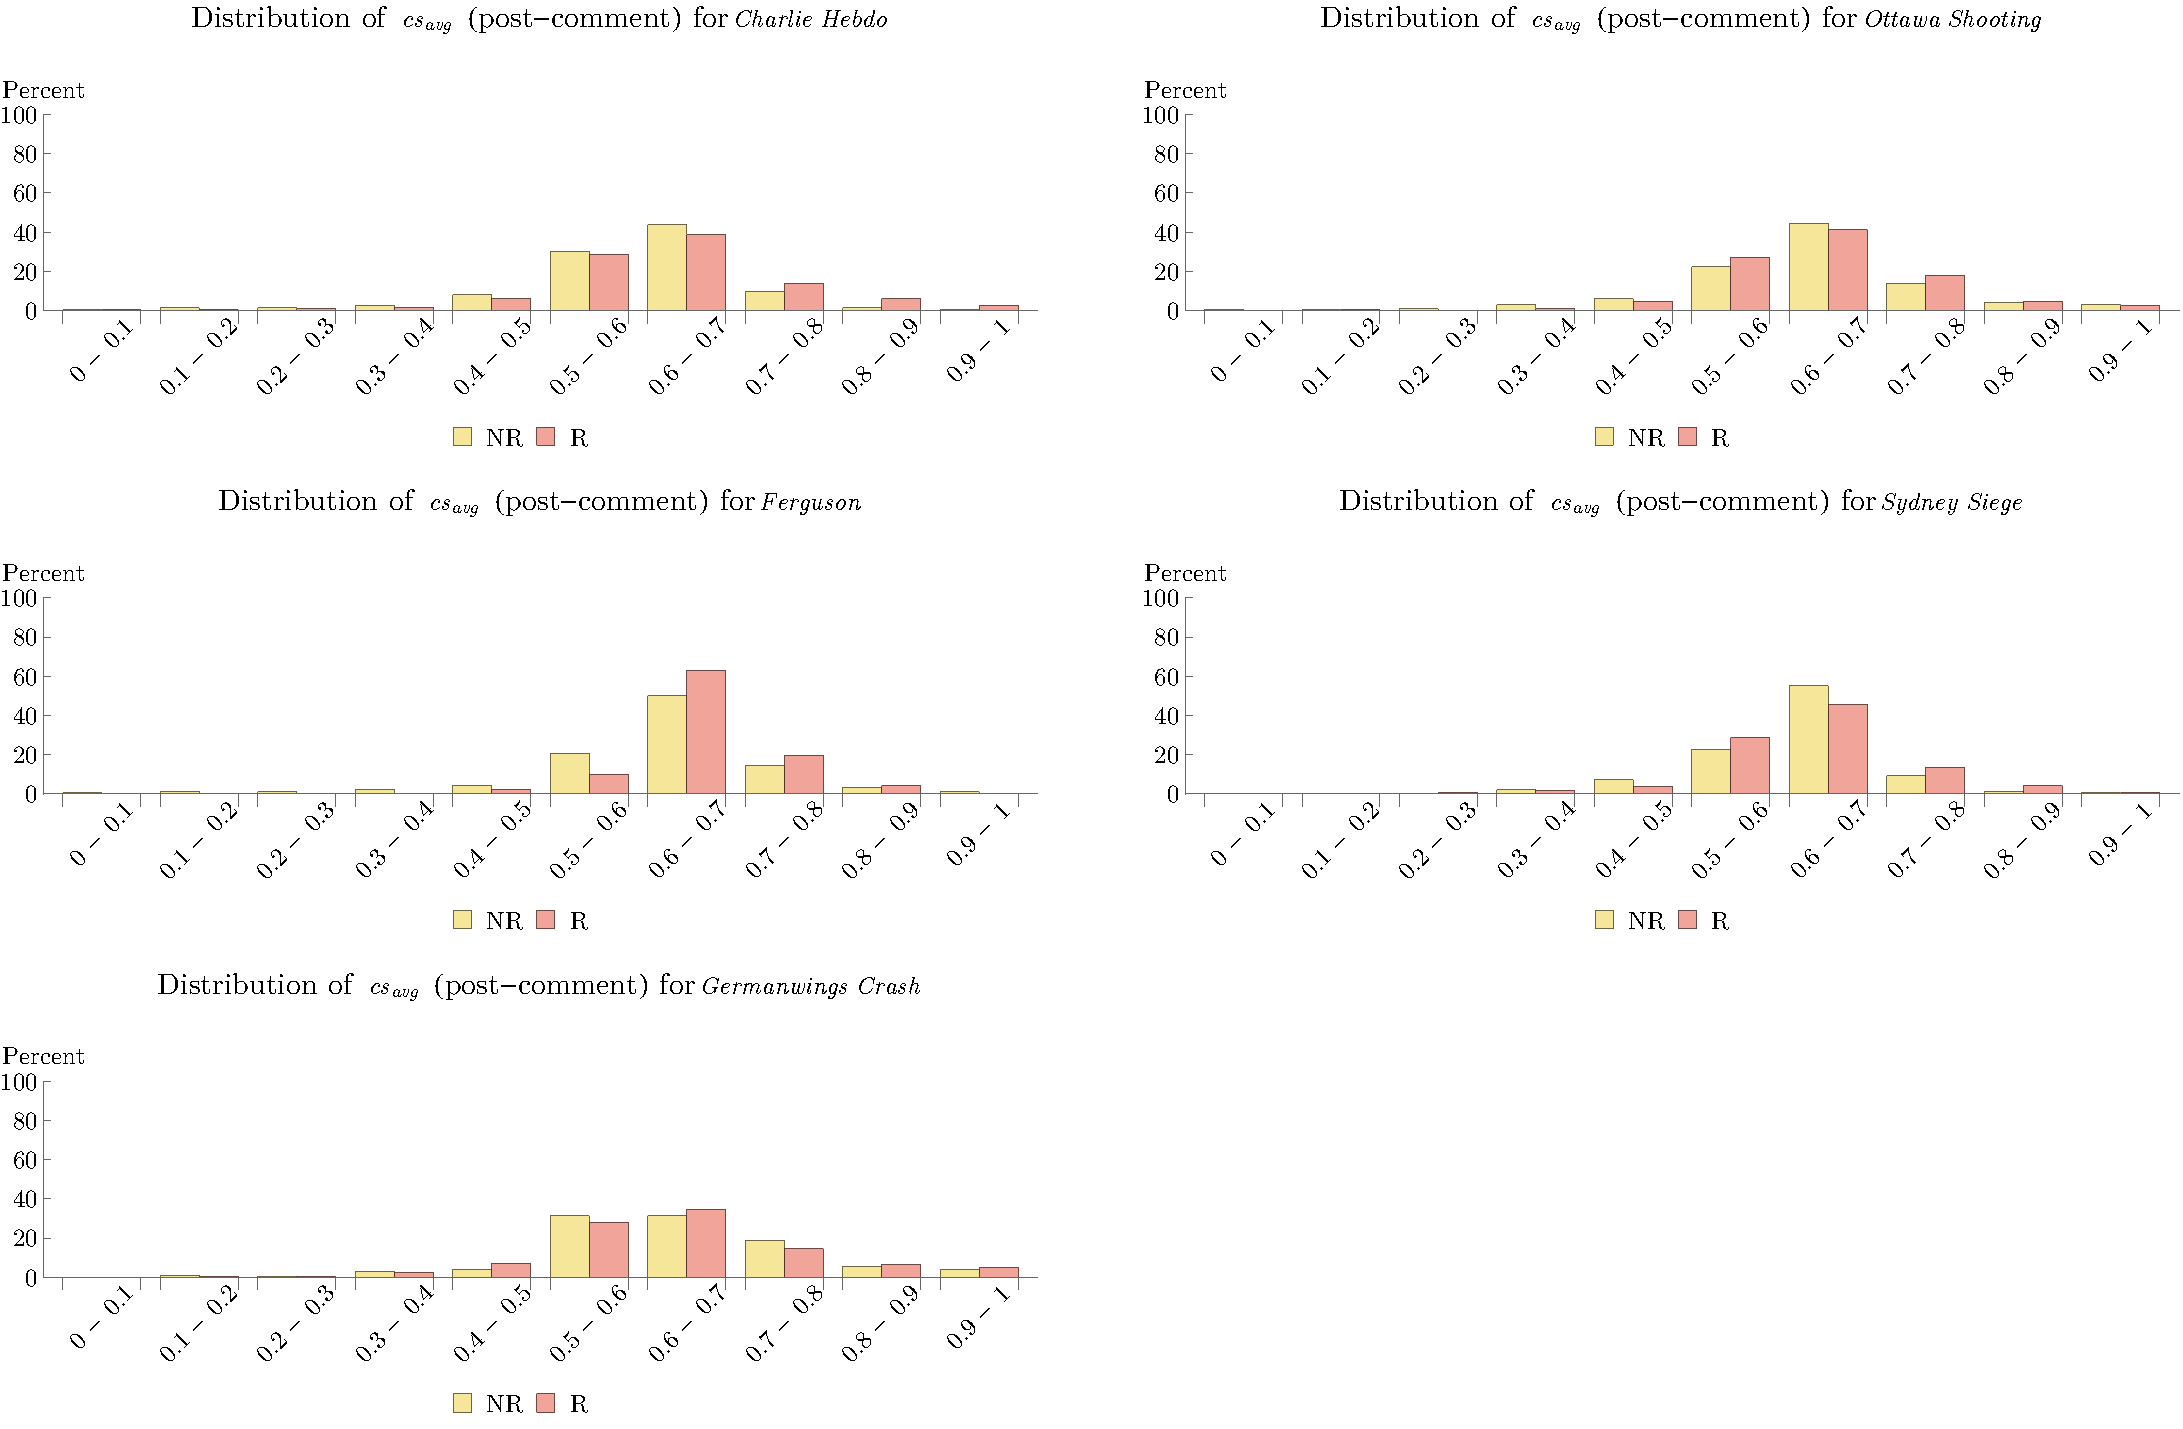
\includegraphics[width={\textwidth + \marginparsep + \marginparwidth}]{gfx/Experiment_1_3}
  % \begin{varwidth}{\textwidth + \marginparsep + \marginparwidth}
  \caption{Distributions of average pairwise cosine similarities between posts and their comments. $NR=\textrm{non-rumours}, R=\textrm{rumours}$.}
  % \end{varwidth}
  \label{fig:3-exp-1.3}
\end{figure}

\begin{figure}[h]
  \myfloatalign
  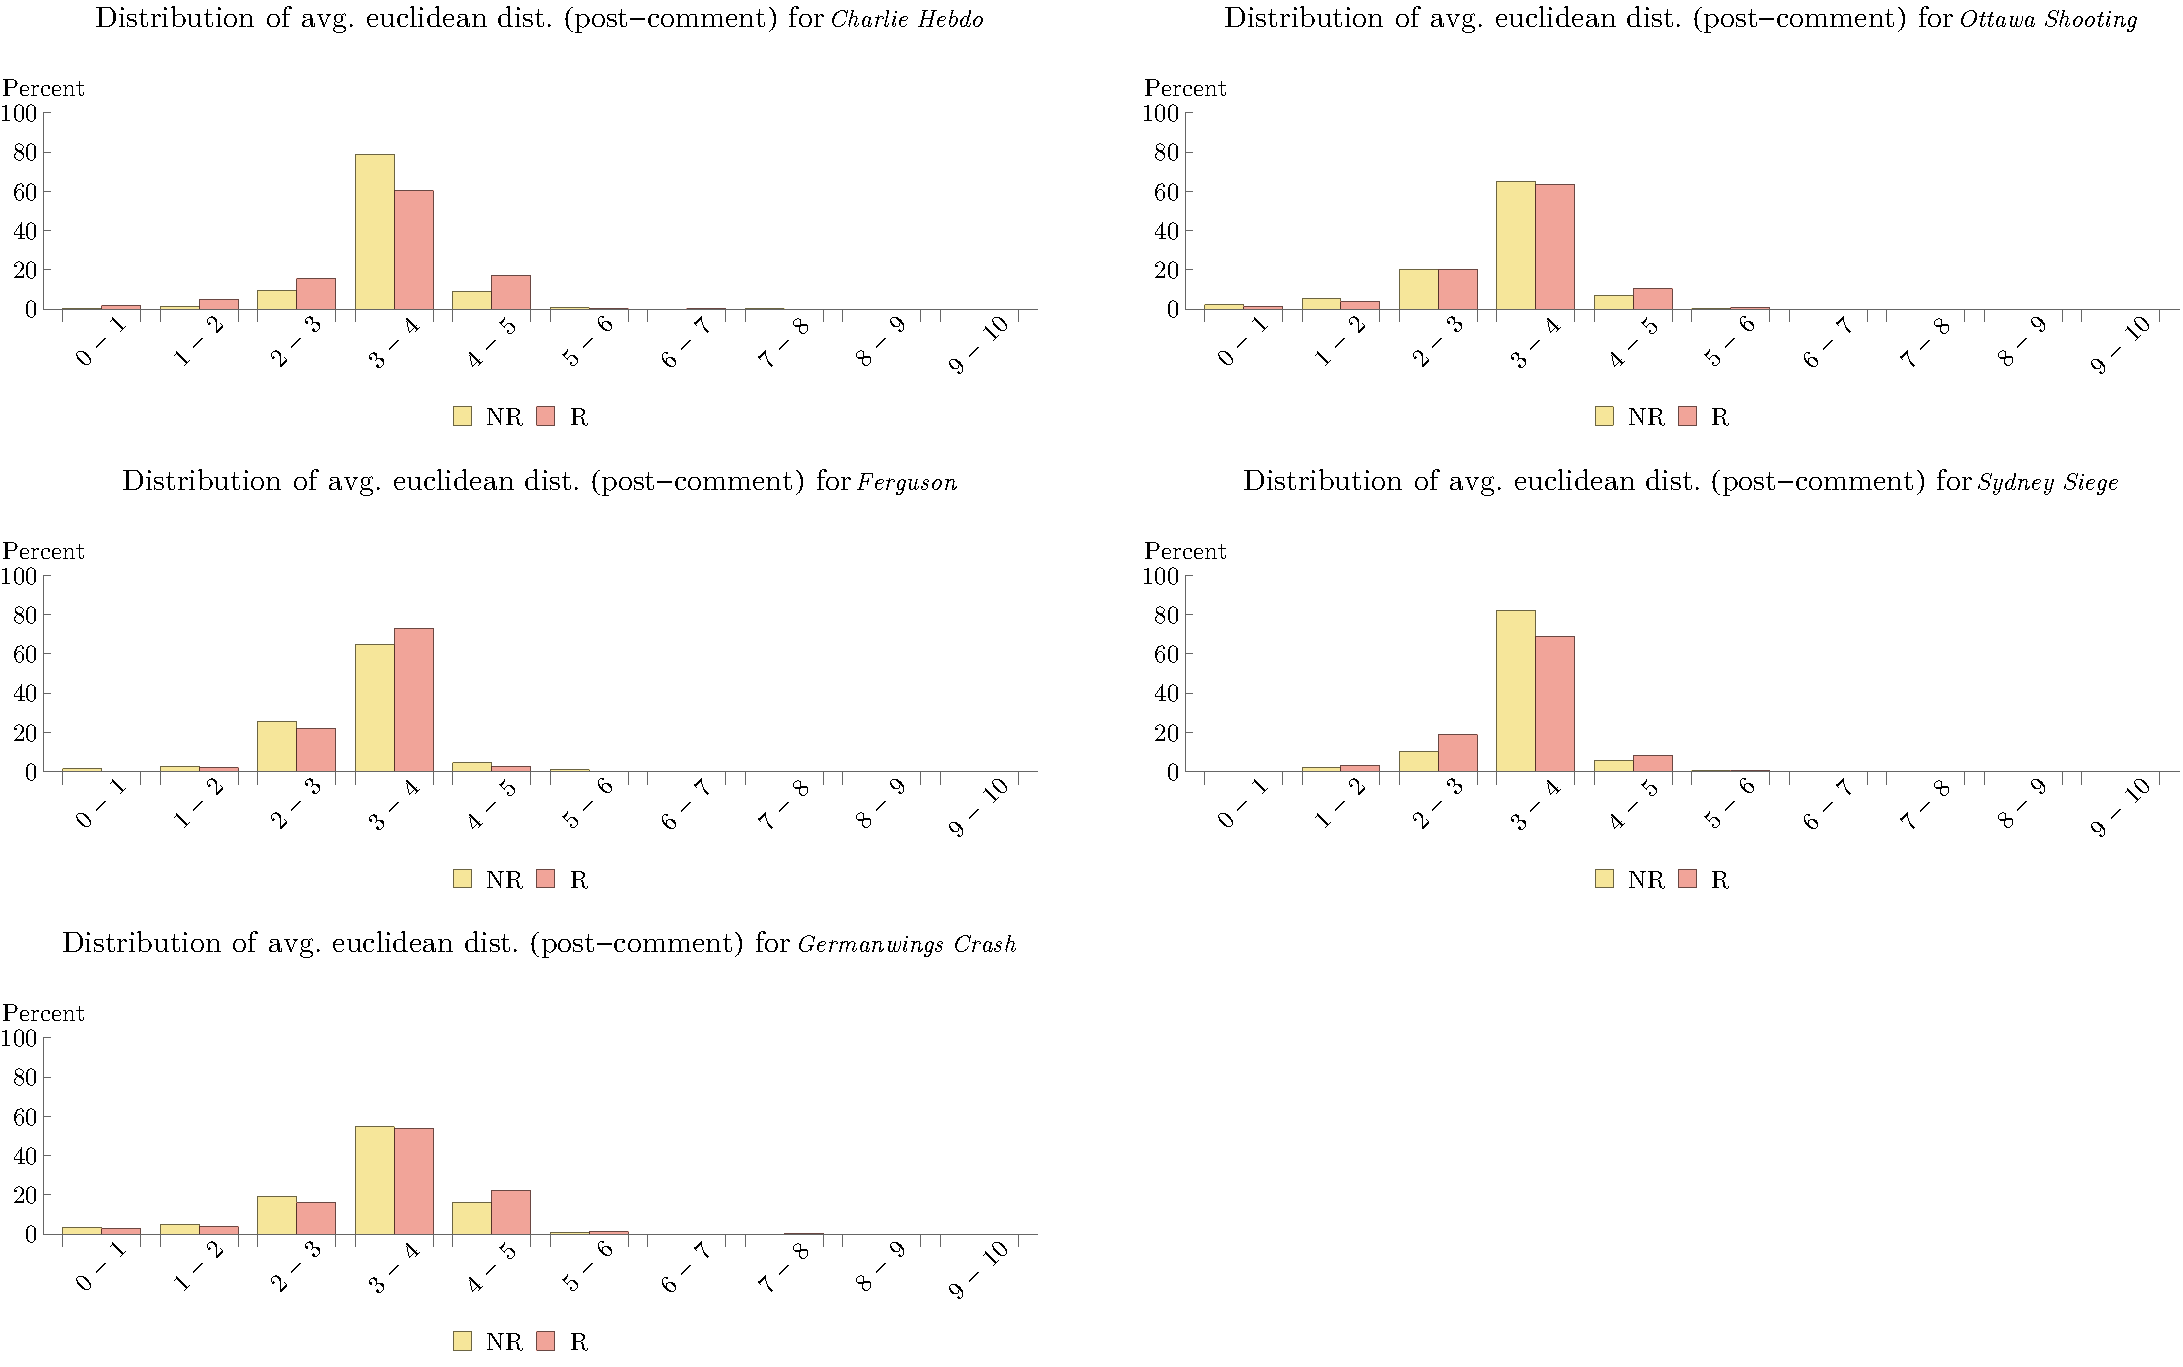
\includegraphics[width={\textwidth + \marginparsep + \marginparwidth}]{gfx/Experiment_1_3_eucl}
  % \begin{varwidth}{\textwidth + \marginparsep + \marginparwidth}
  \caption{Distributions of average pairwise Euclidean distances between posts and their comments. $NR=\textrm{non-rumours}, R=\textrm{rumours}$.}
  % \end{varwidth}
  \label{fig:3-exp-1.3e}
\end{figure}

\begin{table}[h]
\addlinespace
    \begin{tabularx}{\textwidth}{Xl} \toprule
        \tableheadline{Event} & \tableheadline{Euclidean distance} \\ \midrule
        Charlie Hebdo Shooting & -1.365 \\
        Ferguson Unrest & 0.924 \\
        Germanwings Crash & 1.156 \\
        Ottawa Shooting & 0.076 \\
        Sydney Siege & -1.608 \\
        \bottomrule
    \end{tabularx}
\caption{Difference between the averages of the Euclidean distances of rumour and non-rumour comments.}
\label{tab:3-exp-1.3}
\end{table}

\section{Disparities in sentiment }
\label{sec:3-sentiment}

As mentioned earlier (see \sectionref{ssec:1-fnosn}), authors of false news sometimes seek to arouse emotional responses from readers, as has been observed through studies of their writing style. This observation served as the basis for an experiment which aimed to distinguish between rumours and non-rumours by analysing the sentiment expressed in both sets of tweets.

In this experiment, the Stanford NLP tool\sidecite{Socher:2013} was used to analyse the sentiment scores of posts and comments in the PHEME dataset. For a given text, the tool computes one of the following sentiment scores: 0 (very negative), 1 (negative), 2 (neutral), 3 (positive), or 4 (very positive). In the first variant of this experiment, the sentiment scores of the posts and comments of rumour and non-rumour tweets were computed and compared.

The results (plotted in \autoref{fig:3-exp-2.1} and \autoref{fig:3-exp-2.1c}) do not show significant variations between the sentiment scores of rumours and non-rumours, for posts or comments. Further analyses were carried out but the results did not significantly distinguish between rumour and factual comments or posts based on inferred sentiment.

\begin{figure}[h]
  \myfloatalign
  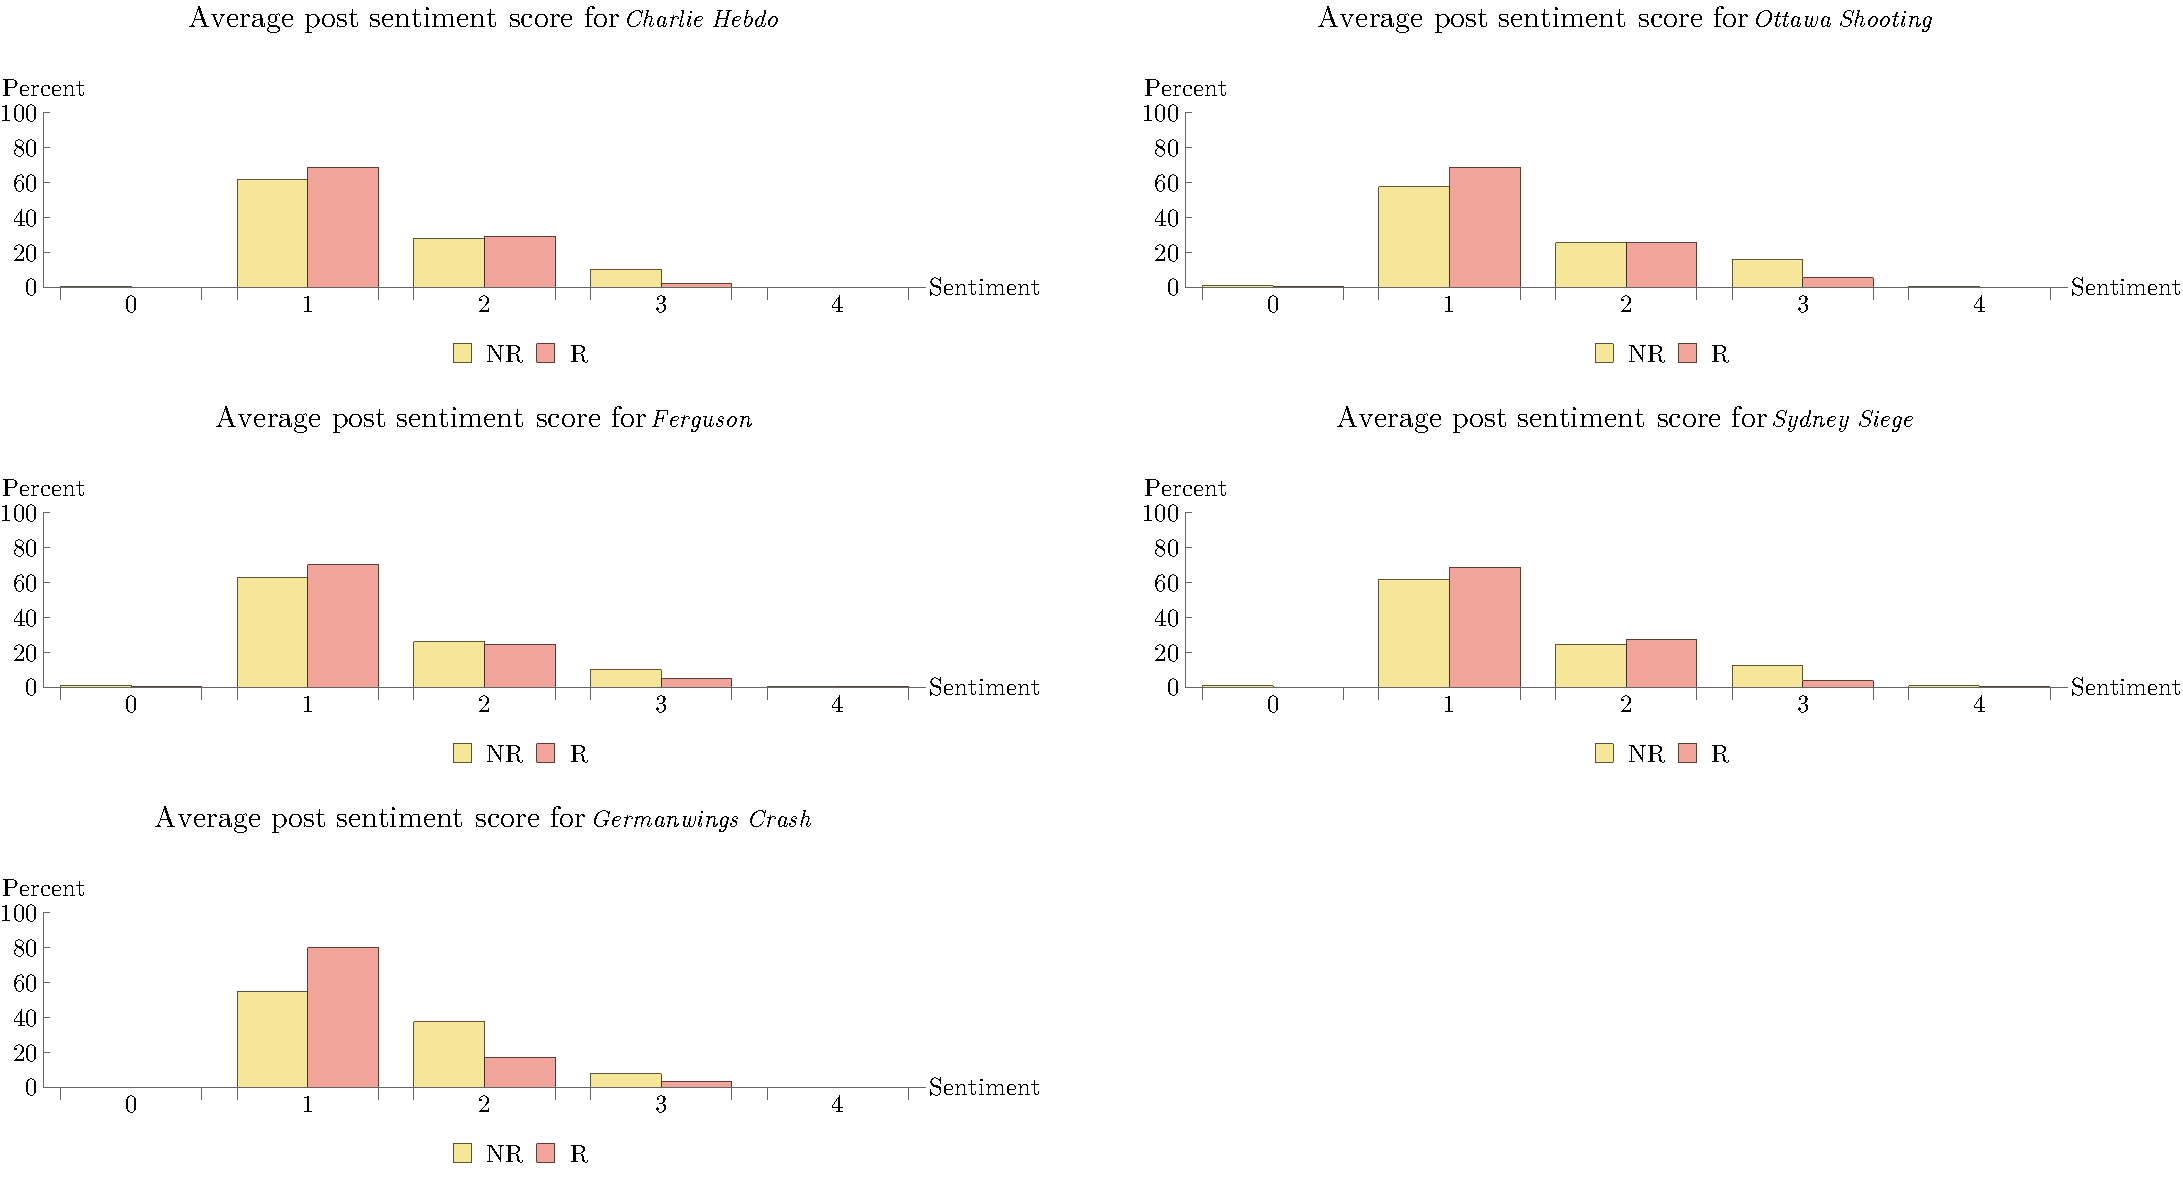
\includegraphics[width={\textwidth + \marginparsep + \marginparwidth}]{gfx/Experiment_2_1}
  % \begin{varwidth}{\textwidth + \marginparsep + \marginparwidth}
  \caption{Average sentiment scores of posts. $NR=\textrm{non-rumours}, R=\textrm{rumours}$.}
  % \end{varwidth}
  \label{fig:3-exp-2.1}
\end{figure}

\begin{figure}[h]
  \myfloatalign
  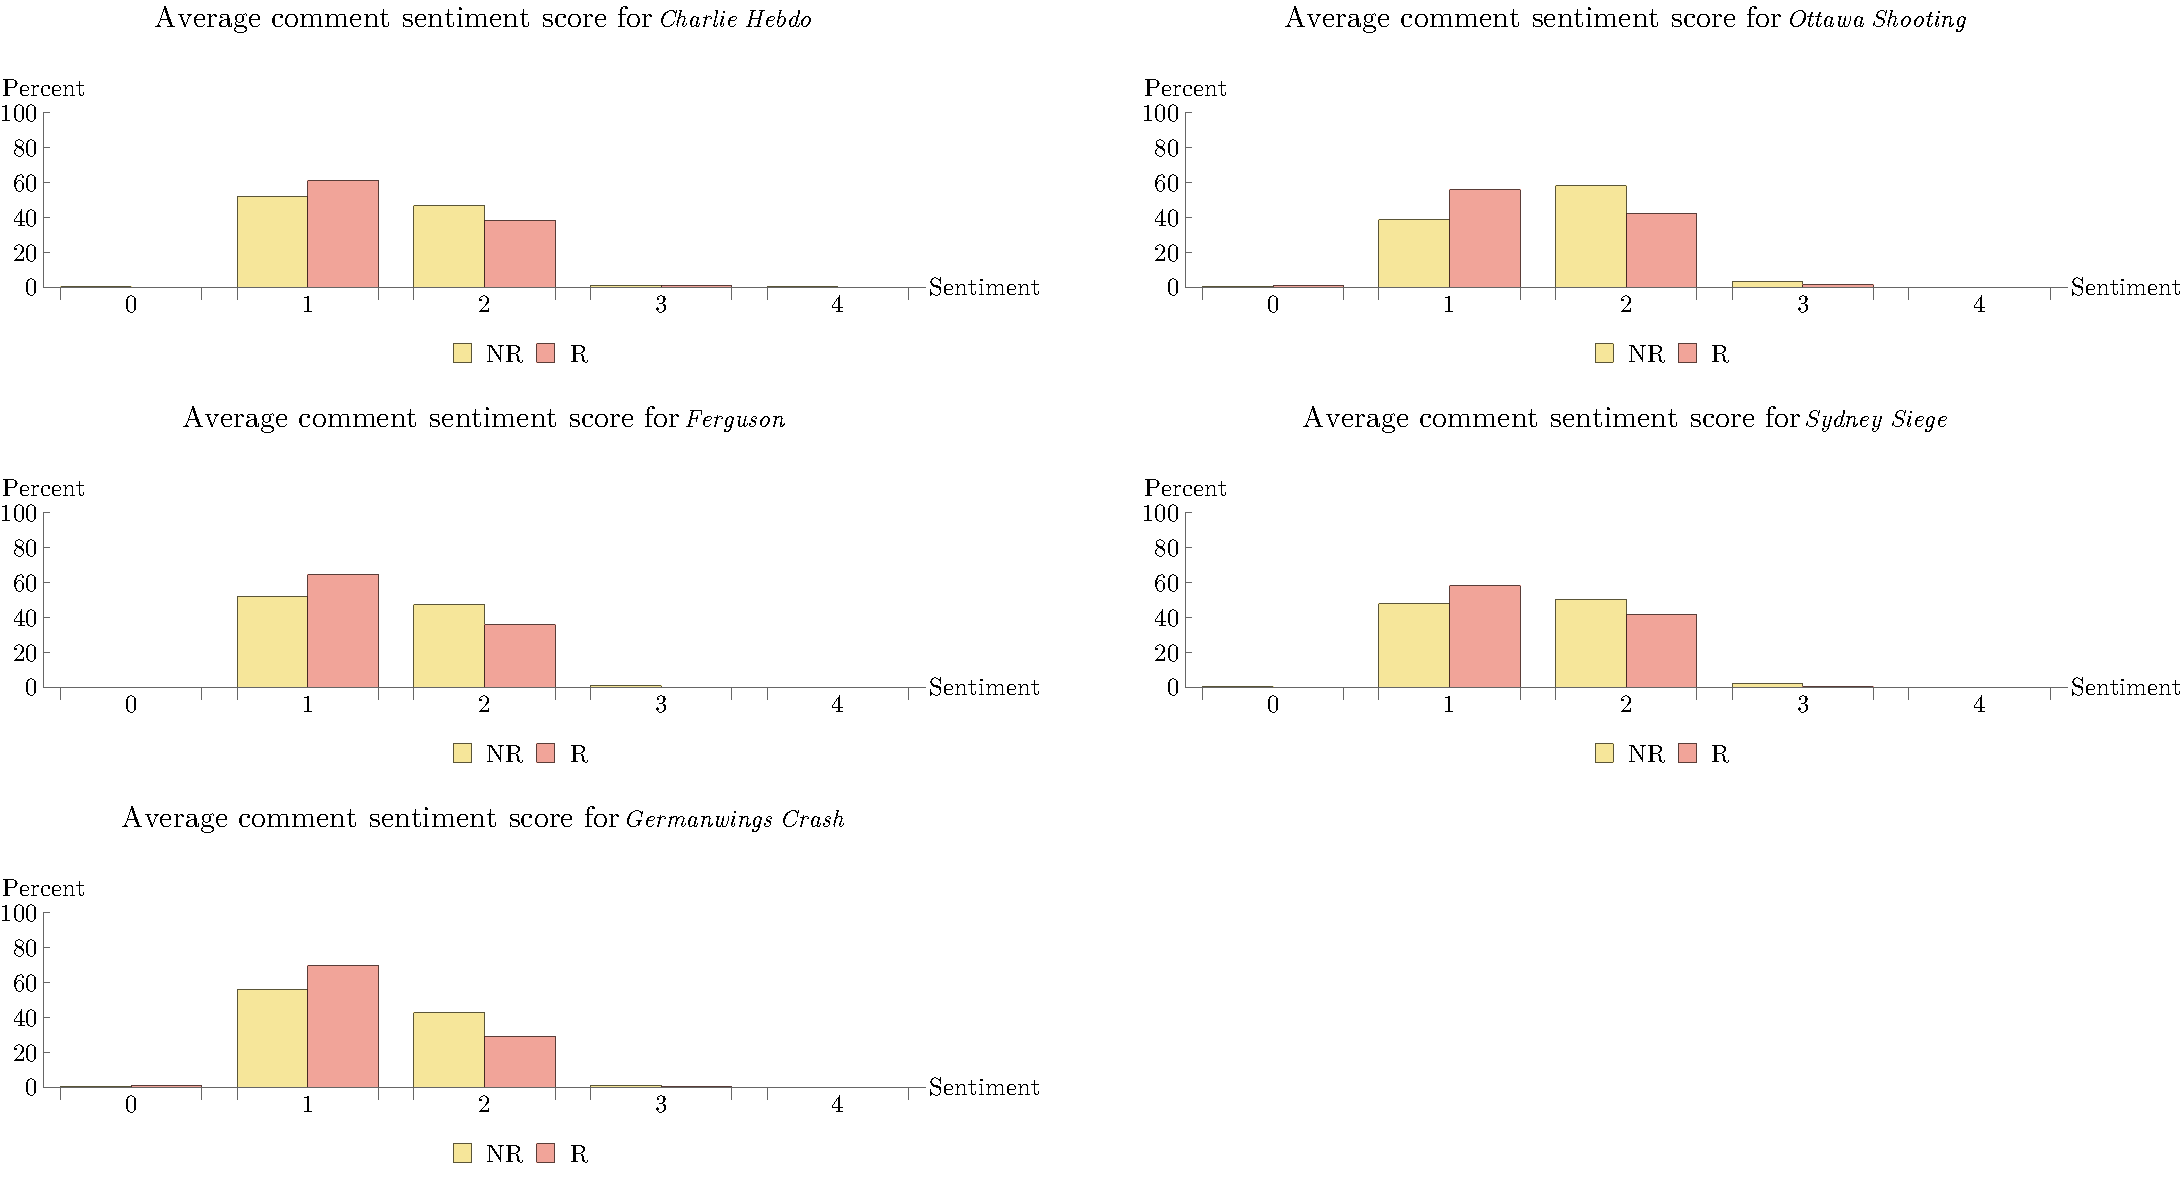
\includegraphics[width={\textwidth + \marginparsep + \marginparwidth}]{gfx/Experiment_2_1_comments}
  % \begin{varwidth}{\textwidth + \marginparsep + \marginparwidth}
  \caption{Average sentiment scores of comments. $NR=\textrm{non-rumours}, R=\textrm{rumours}$.}
  % \end{varwidth}
  \label{fig:3-exp-2.1c}
\end{figure}

\newthought{One final experiment} was performed regarding text embeddings and sentiment. In it, $K$-Means clustering (with $K=2$) was used to analyse the sentiment scores for rumour and non-rumour comments. This was repeated with \texttt{InferSent}, as well as \texttt{word2vec} (300-length vectors) word embeddings, instead of sentiment scores. The results from clustering showed that there is no clear distinction between rumour and non-rumour tweets.

\section{Conclusion}
\label{ssec:3-conclusion}

The series of experiments discussed in this section do not conclude that word or sentence embeddings, or sentiment, can reliably distinguish rumour tweets from factual ones (at least, in the datasets used here), or the reactions that either receive. Nonetheless, these findings are limited, and probably only apply, to the set-up of the experiments presented here. Others have successfully used these text representations in different ways to differentiate between the two types of tweets. To further test the methodology followed here will require substantially larger datasets. Furthermore, as opposed to using simplistic sentiment measures (positive, neutral, and negative), a more granular and precise measure of emotions in tweets can be explored. For example, \citeauthoryear{Vosoughi:2018} examined a range of positive emotions (such as joy and trust) as well as negative ones (such as fear and anger) in both false and true news. They found that comments to false rumours had greater surprise and disgust expressed in them, while reactions to true ones expressed more sadness and anticipation. Similarly, \citeauthoryear{Kolev:2022} carried out fake news detection by using the predicted six emotions (anger, disgust, fear, joy, sadness, and surprise) in the titles of news articles as features.

% end of chapter
